\section{Reactive Design Patterns}

Dieser Teil der Arbeit beschäftigt sich mit Reactive Design Patterns. Dabei handelt es sich nicht um gänzlich neue Design Patterns, sondern vielmehr um Patterns, die sich für die Entwicklung reaktiver Systeme als nützlich erweisen. Der Fokus soll vor allem auf Patterns liegen, die die Eigenschaften reaktiver Anwendungen unterstützen.

\subsection{Observable Pattern}\label{subsec:observable-pattern}
Das reaktive Observable Pattern stammt aus dem Hause Microsoft und wurde von Erik Meijer in dem Framework für reaktive Programming \textit{Reactive Extensions} definiert. Die reaktive Programmierung beschäftigt sich mit dem Datenfluss einer Anwendung und mit der asynchronen Verarbeitung von Events. Bei der Entwicklung von Benutzeroberflächen ist reaktive Programmierung seit langem üblich und verbreitet. Eine Benutzeroberfläche muss stetig auf Eingaben, also Events, durch den Benutzer reagieren. Dazu gehören neben Tastatureingaben und Mausklicks auch Cursorbewegungen. Ebenso können die Anfragen einer Webapplikation als kontinuierlicher Datenstrom aus Events bezeichnet werden.\\
Zu Beginn der Arbeit wurde bereits die Definition reaktiver Systeme genannt. Allgemeiner betrachtet bedeutet das englische Wort \textit{reactive} laut dem Merriam-Webster Wörterbuch \enquote{readily responsive to a stimulus}\footnote{http://www.merriam-webster.com/dictionary/reactive}. Demnach ist etwas \textit{reactive}, wenn es bereitwillig auf einen Reiz reagiert. Im Bezug auf Software sind Reize Events, die von einer Komponente verarbeitet werden müssen \cite{rappl_introduction_2016} \cite[S.~4]{carkci_dataflow_2014} \cite[S.~5]{blackheath_functional_2015}.\\
Für die Verarbeitung von Events nutzt man traditionellerweise das Verhaltensmuster \textit{Observer}. Dieses Muster beschreibt zwei Akteure bzw. Rollen. Das beobachtbare Subjekt, emittiert bzw. veröffentlicht Events. Die Events können von beliebig vielen Empfängern verarbeitet werden. Diese Empfänger werden als Beobachter oder auch als Observer bezeichnet. Ein Observer hat die Möglichkeit sich für Zustandsänderungen des Subjekts an- und abzumelden \cite[S.~293]{gamma_design_1995}.\\
Ein endlicher Strom von Events ist im Grunde nichts anderes als eine Liste. Für die Verarbeitung einer Liste nutzt man traditionellerweise das Verhaltensmuster \textit{Iterator}. Dieses Muster ermöglicht den sequenziellen Zugriff auf Elemente einer aggregierten Datenstruktur. Der Iterator definiert hierfür eine Schnittstelle für den Zugriff und das Traversieren beispielsweise einer Liste \cite[S.~257]{gamma_design_1995}.\\
Die beiden Patterns unterscheiden sich jedoch im Hinblick auf den Zugriff der Daten. Beim Iterator Pattern wird der Iterator nach weiteren Daten gefragt. Man nennt dies Pull-Strategie. Im Gegensatz dazu nutzt man beim Observer Pattern die Push-Strategie. Der Observer wird vom Subjekt benachrichtigt, falls weitere Daten verarbeitet werden müssen. Das Observer Pattern hat im Vergleich zum Iterator Pattern zwei Nachteile. Das Pattern beschreibt keine Möglichkeit einer Fehlerbehandlung und auch die Mitteilung, dass keine weiteren Events mehr eintreffen werden, ist nicht vorgesehen.\\
Das Observable Pattern kombiniert beide Patterns. Zum einen verwendet es die Push-Strategie und das Beobachten des Observer Patterns. Zum anderen kann ein Observable für das Ende des Datenstroms sowie über Fehler informiert werden. Ein Subscriber eines Observables definiert eine Schnittstelle mit den drei folgenden Methoden \cite{reactivex_2014}:

\begin{enumerate}
\item \textit{onNext(Event)}\\
Wird aufgerufen, falls ein Event verarbeitet werden soll.
\item \textit{onError(Exception)}\\
Wird aufgerufen, falls etwa beim Aggregieren ein Fehler aufgetreten ist.
\item \textit{onCompleted()}\\
Wird aufgerufen, falls das Ende des Datenstroms erreicht ist.
\end{enumerate}

Observables abstrahieren den Datenfluss und durch die Observer Eigenschaften können Implementierungsdetails, wie beispielsweise \gls{concurrency} versteckt werden. Zudem wird eine asynchrone und nicht blockierende Verarbeitung von Events ermöglicht \cite[S.~81]{kuhn_reactive_2015}.

\pagebreak

\begin{lstlisting}[caption={Zusammenknüpfen und filtern zweiter Listen mit RxJava},label={lst:rxjava}]
List<String> w = Arrays.asList("Anna", "Eva", "Andrea", "Christiane");
List<String> m = Arrays.asList("Martin", "Tom", "Leon", "Alexander");
Observable.concat(Observable.from(w), Observable.from(m))
 .filter(name -> name.startsWith("A"))
 .subscribe(new Subscriber<String>() {
   public void onCompleted() {
    System.out.println("Completed");
   }
   public void onError(Throwable throwable) {
    System.err.println("Error");
   }
   public void onNext(String name) {
    System.out.println("Name: "+name);
   }
 });
\end{lstlisting}

Das Beispiel zeigt die Verwendung der Reactive Extensions für Java\footnote{RxJava (https://github.com/ReactiveX/RxJava)}. Es werden zwei Listen mit weiblichen und männlichen Vornamen verbunden (Zeile~3). Der daraus resultierende Datenstrom von Vornamen wird nach Namen gefiltert, welche mit \enquote{A} beginnen (Zeile~4). Zum Schluss wird ein Subscriber implementiert, welcher die Namen ausgibt.\\
Anstelle der zwei Listen ist es auch möglich Anfragen von einem Socket abzuarbeiten. Die einzelnen Funktionen, wie der Filter oder auch der Subscriber können wiederverwendet und anderweitig kombiniert werden.\\

Observables eignen sich sehr gut, um Datenströme asynchron zu verarbeiten. Die Reactive Extensions sind in ereignisbasierten Anwendungen (siehe \ref{subsec:eventdriven-concurrency}) von großem Nutzen. Für die Entwicklung von, durch Nachrichten gesteuerte, reaktive Applikationen sind die Reactive Extensions deshalb sehr nützlich. Jedoch wird durch deren Verwendung keine der vier reaktiven Eigenschaften direkt erfüllt \cite[S.~82]{kuhn_reactive_2015}.

\pagebreak

\subsection{Simple Component Pattern}\label{subsec:simple-component-pattern}
Ein umfangreiches System erledigt meist mehrere Aufgaben und hat verschiedenste Funktionalitäten. Die einzelnen Funktionen sollten isoliert voneinander betrachtet werden. Folglich empfiehlt es sich, die Software in einzelne Komponenten aufzuteilen. Die Komplexität des großen Ganzen, wird hiermit auf viele kleinere Komponenten heruntergebrochen.\\
Sind die Komponenten funktional voneinander isoliert, bedarf es bei der Entwicklung weniger Abstimmung zwischen den jeweiligen Teams hinter einer Komponente. Die Komponenten können unabhängig voneinander weiterentwickelt werden \cite[S.~215]{newman_building_2015}.\\
Dieses Pattern trägt den Namen Simple Component und wird wie folgt definiert:

\begin{quotation}
A component shall do only one thing, but do it in full \cite[S.~185]{kuhn_reactive_2015}.
\end{quotation}

Beispielsweise kann ein Textbearbeitungsprogramm mit Rechtschreibprüfung in Textbearbeitung und Rechtschreibprüfung aufgeteilt werden. Die Rechtschreibprüfung ist nicht abhängig von der eigentlichen Textbearbeitung und umgekehrt \cite[S.~185]{kuhn_reactive_2015}. Ein anderes Beispiel wäre ein Onlineshop. Ein Onlineshop besteht unter anderem aus folgenden Komponenten:

\begin{enumerate}
\item Produktverwaltung
\item Kundenverwaltung
\item Kundenauthentifizierung
\item Warenkorb \& Bestellvorgang
\item Zahlungsabwicklung
\end{enumerate}

Die Liste beansprucht keine Vollständigkeit und zeigt trotzdem, dass einzelne Komponenten keinesfalls trival sein müssen aber im Vergleich zu der gesamten Anwendung simpler sind.

\pagebreak

Das Pattern ist keineswegs neu. Es kann aus dem \textit{Single Responsibility Priniciple} von Robert C. Martin abgeleitet werden. Das Prinzip zielt auf objektorientierte Systeme ab und lautet: \enquote{A class should have only one reason to change}. Befolgt man dieses Prinzip maximiert man die Kohäsion und minimiert die Kopplung zwischen Klassen --- oder auch zwischen Komponenten \cite[S.~185]{kuhn_reactive_2015} \cite{martin_single_2014}.\\
Eine weitere Definition in diesem Zusammenhang stammt von Rotem-Gal-Oz bezüglich eines Services in einer Service-orientierten Architektur:

\begin{quotation}
[...] a service should provide a distinct business function [...]. One of the characteristics of services is \textit{service autonomy}, which means the service should be mainly self-sufficient \cite[S.~7]{rotem_soa_2012}.
\end{quotation}

Ein Service oder im übertragenen Sinn eine Komponete sollte, falls möglich, autark und unabhängig sein. Folglich empfiehlt es sich die Logik einer Funktionalität nicht über mehrere Komponenten aufzuteilen.\\

Ein System im Ganzen betrachtet ist sehr komplex und schwer zu fassen. Mithilfe des Simple Component Patterns bricht man das System Schritt für Schritt in einzelne Verantwortlichkeiten und somit in einzele Komponenten auf. Es entsteht eine Hierarchie aus Komponenten und Unterkomponenten, die voneinander isoliert betrachtet werden können.\\
Das Simple Component Pattern ist ein grundlegendes und elementares Reactive Design Pattern. Folgt man dem Pattern können die reaktiven Prinzipien \textit{supervision} (\ref{subsec:actor-model}) und \textit{share nothing} (\ref{subsec:sharenothing}) umgesetzt werden. Schlussendlich ermöglicht dieses Pattern, Komponenten von einander zu isolieren und dies wiederum unterstützt bei der Umsetzung der geforderten reaktiven Eigenschaft \textit{resilience} (\ref{subsec:resilient}).

\pagebreak

\subsection{Let-It-Crash Pattern}\label{subsec:let-it-crash-pattern}
Beim Entwurf reaktiver Software wird von vornherein angenommen, dass das System durch Hardware- und/oder Softwarefehler ganz oder teilweise ausfallen kann. Ein reaktives System muss gegenüber Ausfällen \textit{resilience} vorweisen können (siehe \ref{subsec:resilient}).\\
Durch die Komponentenhierarchie, die durch das \nameref{subsec:simple-component-pattern} entsteht, ist es möglich untergeordnete Komponenten in ihrem Lebenszyklus zu beeinflussen.\\
Tritt in einer Komponente ein zufälliger Fehler auf, versucht nicht die Komponente selbst den Fehler zu beheben, sondern lässt deren Supervisor den Fehler behandeln \cite[S.~196]{kuhn_reactive_2015} \cite[S.~200~\&~S.~201]{armstrong_programming_2013}. Die eigentliche Logik und die Fehlerbehandlung sind somit entzerrt. Treten zufällige oder seltene Fehler auf, wie beispielsweise ein ungewöhnlicher Fehlerzustand oder ein blockierter Datenbank-Connection-Pool, wird die Komponente durch den Supervisor neugestartet. Der interne Zustand wird somit zurückgesetzt und zuvor gebundene Ressourcen (z.B. File-Handles, Datenbankverbindungen) werden freigegeben \cite[S.~197]{kuhn_reactive_2015}. Fehler, wie beispielsweise falsche oder fehlende Parameter sind hiervon ausgenommen und führen nicht zu einem Neustart.\\
Das beschriebene Prinzip nennt sich Let-It-Crash Pattern und wird folgendermaßen definiert:

\begin{quotation}
Prefer a full component restart to a complex internal~failure~handling~\cite[S.~196]{kuhn_reactive_2015}.
\end{quotation}

Man verzichtet somit auf aufwendige Fehlerbehandlung innerhalb einer Komponente und zieht es vor, dass eine fehlerhafte Komponente jederzeit durch den Supervisor beendet werden kann. Der Supervisor kann darüber hinaus weitere Maßnahmen, wie beispielsweise Load Balancing, ergreifen, um fehlerhafte Nodes oder Komponenten zu umgehen.

\pagebreak

Das Let-It-Crash Pattern hat Einfluss auf die Verfügbarkeit des Systems. Die Verfügbarkeit lässt sich aus folgenden Zeitwerten berechnen \cite{friedrichsen_unkaputtbar_2014}:

\begin{enumerate}
\item MTTF (\textit{Mean Time To Failure}) beschreibt die durchschnittliche Zeit bis zum Auftreten eines Fehlers.
\item MTTR (\textit{Mean Time To Recovery}) beschreibt die durchschnittliche Zeit bis zur vollständigen funktionalen Wiederherstellung des Systems.
\end{enumerate}

Diese zwei durchschnittlichen Zeitwerte stehen wie folgt in Zusammenhang:

\begin{figure}[H]
\[Availability := \frac{MTTF}{MTTF + MTTR}\]
\caption{Formel zur Berechnung der Verfügbarkeit}
\end{figure}

Die Verfügbarkeit, in der Formel \textit{Availability} genannt, sollte einen Wert gegen 1 erreichen. Bei der Verfügbarkeit handelt es sich um den prozentualen Zeitanteil in der eine Software das tut, was sie tun soll \cite[S.~11]{hanmer_patterns_2007}.\\
Der traditionelle Ansatz ist, die MTTF zu maximieren und somit die MTTR zu vernachlässigen. Wie bereits festgestellt wurde, lassen sich Fehler nicht ausschließen. Der Let-It-Crash Ansatz, konzentriert sich vielmehr auf die MTTR und versucht diese soweit wie möglich zu minimieren \cite[S.~198]{kuhn_reactive_2015} \cite{friedrichsen_unkaputtbar_2014}.\\

Das Let-It-Crash Pattern muss, wie auch das Simple Component Pattern (\ref{subsec:simple-component-pattern}), bereits beim Design der Anwendung berücksichtigt werden. Es trägt dazu bei, die \textit{resilience} eines reaktiven Systems zu erhöhen und unterstützt somit auch ganz klar die \textit{responsiveness}.

\pagebreak

\subsection{Heartbeat Pattern}\label{subsec:heartbeat-pattern}
Durch Supervision in einer Komponentenhierarchie und dem Let-It-Crash Pattern (\ref{subsec:let-it-crash-pattern}) kann in einer reaktiven Anwendung auf explizite und definierte Weise mit Fehlerzuständen umgegangen werden. Jedoch stellt sich nun die Frage, wie Supervisor effektiv die Fehler der untergeordneten Komponenten feststellen können.\\
Dazu ist es wichtig zu wissen, welche Fehler eintreten bzw. in welche Kategorien Fehler eingeteilt werden \cite{friedrichsen_unkaputtbar_2014}.

\begin{enumerate}
\item \textbf{Crash Failure} (Absturzfehler)\\
Die Komponente antwortet nicht mehr, da es durch Hard- oder Softwarefehler zu einem Absturz kam.
\item \textbf{Omission Failure} (Auslassungsfehler)\\
Die Komponente reagiert auf vereinzelte Anfragen nicht, da diese Anfragen nie ankamen oder deren Antwort verloren ging.
\item \textbf{Timing Failure} (Antwortzeitfehler)\\
Die vereinbarte maximale Antwortzeit wurde überschritten (Timeout).
\item \textbf{Response Failure} (Antwortfehler)\\
Die Antwort ist fehlerhaft oder schlichtweg falsch.
\item \textbf{Byzantine Failure} (Zufälliger Fehler)\\
Die Komponente verhält sich zu unbestimmten und zufälligen Zeitpunkten fehlerhaft.
\end{enumerate}

Eine einfache Möglichkeit den Zustand bzw. die Verfügbarkeit einer Komponente zu überprüfen, ist das Heartbeat Pattern. Der Supervisor schickt in regelmäßigen Abständen spezielle Anfragen, die die Komponente auffordert ein Lebenszeichen, einen sogenannten Heartbeat, von sich zu geben. Erhält der Supervisor auf die Anfrage keine Antwort, kann nach Ablauf eines Timeouts, mit großer Wahrscheinlichkeit von einem Crash Failure ausgegangen werden \cite[S.~200~\&~S.~201]{kuhn_reactive_2015}.\\
Die Komponente kann die Heartbeat Nachricht auch mit Informationen über deren Zustand erweitern, wie beispielsweise Fehlerrate oder Zahl der Anfragen.\\
Das Heartbeat Pattern kann aus der Sicht der Komponente aktiv oder passiv umgesetzt werden. Das heißt die Komponente sendet die Heartbeat Nachricht auf Anfrage an den Supervisor oder selbstständig in regelmäßigen Abständen an eine vereinbarte Adresse. Sendet die Komponente die Heartbeats selbstständig, muss der Supervisor trotzdem prüfen, ob in gewissen Zeitabständen ein Heartbeat der überwachten Komponente eingeht. Der Supervisor ist somit nach wie vor in der Verantwortung Fehler zu erkennen.\\

Eine weitere Möglichkeit den Zustand einer Komponente im System verfügbar zu machen sind pro-aktive Failure Signals. Stellt die Komponente einen Fehler fest, kann ähnlich zum aktiven Heartbeat eine Nachricht mit Informationen über den Fehler an eine vereinbarte Addresse geschickt werden \cite[S.~201~\&~S.202]{kuhn_reactive_2015}. Die Fehlerbehandlung sollte dann jedoch dem Supervisor überlassen werden.\\
Durch pro-aktive Failure Signals können Fehler der Kategorien 2. bis 5. an den Supervisor gemeldet werden. Jedoch sollte man beachten, dass die Komponente möglicherweise nicht jeden Fehler selbst erkennt und die Failure Signals aufgrund von Störungen in der Kommunikation nicht beim Supervisor eintreffen.\\

Das Heartbeat Pattern ermöglicht es, Crash Failures über die Hierarchie Ebenen hinweg festzustellen. Durch die Erweiterung des Heartbeat Patterns mit pro-aktiven Failure Signals können auch andere Fehlerkategorien erkannt werden --- jedoch nicht mit 100-prozentiger Garantie. Das Heartbeat Pattern kann ebenfalls zu den \textit{resilience} Patterns gezählt werden. 

\pagebreak

\subsection{Circuit Breaker Pattern}\label{subsec:circuit-breaker-pattern}
Im Zuge der Erläuterung des Heartbeat Pattern (\ref{subsec:heartbeat-pattern}) wurde deutlich, dass die Fehlererkennung für bestimmte Fehlerkategorien unterschiedlich abläuft und nicht immer von der Komponente selbst übernommen werden kann. Der Supervisor muss Anfragen und deren Antworten auf Omission, Timing, Response und Byzantine Failures prüfen.\\
Das Circuit Breaker Pattern ist eine Möglichkeit diese Fehlererkennung zu abstrahieren und in einer allgemeinen Form zur Verfügung zu stellen. Der Begriff Circuit Breaker, auf Deutsch Schutzschalter oder auch Überlastungschutz, stammt aus der Elektrotechnik und dient als Schutz für ein Stromnetz vor Überlastung durch beispielweise einen Kurzschluss \cite[S.~93]{nygard_release_2007}.\\
Kuhn beschreibt das Circuit Breaker Pattern mit folgenden Worten:

\begin{quotation}
Protect services by breaking the connection to their users during prolonged failure conditions \cite[S.~202]{kuhn_reactive_2015}.
\end{quotation}

Wird das Circuit Breaker Pattern angewandt, bedeutet dies, dass der Nachrichtenfluss zwischen zwei Komponenten durch einen Circuit Breaker geschleust wird. Der Circuit Breaker ist zunächst im geschlossenem Zustand (siehe Abb. \ref{fig:circuit-breaker-closed}) und lässt jede Nachricht und deren Antwort zu \cite[S.~93]{nygard_release_2007}.

\begin{figure}[H]
 \centering
 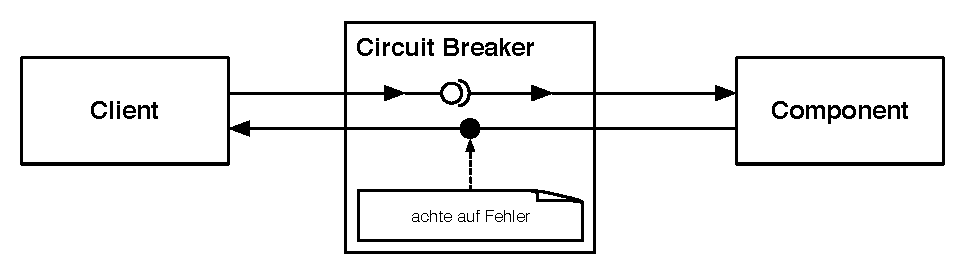
\includegraphics[width=1.0\textwidth]{4-Hauptteil/circuit-breaker/circuit-breaker-closed.eps}
 \caption{Circuit Breaker im geschlossenem Zustand.}
 \label{fig:circuit-breaker-closed}
\end{figure}

Ist die Kommunikation zwischen den Komponenten erfolgreich, bleibt der Circuit Breaker im geschlossenem Zustand. Im Fehlerfall hat der Circuit Breaker die Möglichkeit, den Nachrichtenfluss absichtlich zu unterbrechen. Wird der Nachrichtenfluss unterbrochen, befindet sich der Circuit Breaker im offenem Zustand (siehe Abb. \ref{fig:circuit-breaker-open}). In diesem Zustand wird jede Anfrage sofort mit einer negativen Rückmeldung quittiert --- ohne eine Anfrage verschickt zu haben \cite[S.~94]{nygard_release_2007}.

\begin{figure}[H]
 \centering
 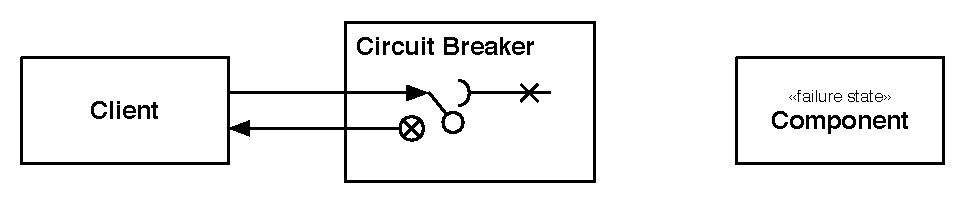
\includegraphics[width=1.0\textwidth]{4-Hauptteil/circuit-breaker/circuit-breaker-open.eps}
 \caption{Circuit Breaker im offenem Zustand.}
 \label{fig:circuit-breaker-open}
\end{figure}

Der Circuit Breaker überwacht Antworten sowie Antwortzeiten und protokolliert die Fehler der Kommunikation. Je nach Konfiguration wird die Verbindung, beispielsweise nach 5 fehlerhaften Antworten, absichtlich unterbrochen \cite[S.~94]{nygard_release_2007}.\\
Gründe für den offenen Zustand können beispielsweise Überlastung oder fehlerhaftes Verhalten der angefragten Komponente sein. Überlastung kann dazu führen, dass die Antwortzeiten stetig steigen, bis hin zu Timing oder Omission Failures. Wird die Verbindung unterbrochen, kann sich die überlastete Komponente erholen \cite[S.~203]{kuhn_reactive_2015}. Häufige aufeinanderfolgende Response oder Byzantine Failures können ebenfalls Gründe für den offenen Zustand des Circuit Breaker sein.\\
Nach einer definierten Dauer im offenem Zustand, wird der Circuit Breaker in den halb-offenen Zustand versetzt. In diesem Zustand wird eine Testanfrage zugelassen. Ist diese Anfrage erfolgreich, wird der Circuit Breaker in den geschlossenen Zustand gesetzt. Andernfalls fällt der Circuit Breaker zurück in den offenen Zustand \cite[S.~94]{nygard_release_2007}.\\

Das Pattern eignet sich sehr gut, um die Kommunikation zwischen den Komponenten zu entkoppeln. Somit unterstützt es auch die Isolierung von Komponenten. Kombiniert mit dem Heartbeat Pattern können alle Fehlerkategorien abgedeckt werden. Aus der Sicht des Reactive Manifestos trägt das Circuit Breaker Pattern zur \textit{resilience} bei.

\pagebreak

\subsection{Fail Fast Pattern}\label{subsec:fail-fast-pattern}
Eine reaktive Applikation muss \textit{responsive} sein. Das heißt, die Anwendung muss zu jederzeit auf jede Anfrage so schnell wie möglich reagieren. Langsame Antworten sind schlecht für das Nutzungserlebnis. Noch schlechter sind langsame und fehlerhafte Antworten bzw. Fehlermeldungen. Der Nutzer oder auch die Client-Software ist gezwungen auf Antworten zu warten, die schlussendlich fehlerhaft sind.\\
Ein System sollte vorab prüfen, ob es während der Bearbeitung einer Anfrage zu möglichen Fehlern kommen kann. Eben dieses Prinzip beschreibt das Fail Fast Pattern. Eine reaktive Applikation sollte im Fehlerfall schnellstmöglich antworten. Hiermit wird unnötige Ressourcenbindung sowohl auf der Clientseite als auch auf der Serverseite vermieden. Es ist sehr schwer festzustellen bzw. zu beweisen, dass eine Software fehlerfrei ist. Das Fail Fast Pattern erwartet keinen Beweis und ist viel einfacher umzusetzen, als man annehmen könnte \cite[S.~106~\&~S.~107]{nygard_release_2007}.\\
Vor der Durchführung einer Anfrage, sollte eine Applikation prüfen, ob alle benötigten Ressourcen zur Verfügung stehen. Beispielsweise sollte überprüft werden, ob die Datenbank oder andere externe Dienste erreichbar sind. Hierfür eignet sich vor allem das bereits erwähnte Circuit Breaker Pattern (\ref{subsec:circuit-breaker-pattern}). Ist der Circuit-Breaker für die Datenbank-Kommunikation offen, kann eine Anfrage, welche die Datenbank benötigt, sofort mit einer Fehlermeldung abgewiesen werden. Nygard beschreibt dies in einem anschaulichen Beispiel \cite[S.~106]{nygard_release_2007}:

\begin{quotation}
Ein Koch bereitet vor dem Kochen erst einmal alle Zutaten vor --- während dem Kochen festzustellen, dass eine Zutat fehlt, ist sehr ungünstig.
\end{quotation}

Eine weitere Möglichkeit Fehler schnellstmöglich zu erkennen, ist die Überprüfung der Parameter einer Anfrage, bevor Ressourcen angefragt oder gebunden werden. Die Überprüfung sollte so einfach, wie möglich sein und keine aufwendige Berechnung oder Business Logik nach sich ziehen. Dazu gehört unter anderem die Prüfung auf \enquote{not null} oder richtige Formate bzw. richtige Datentypen. Nicht erst durch die Datenbankanfrage sollten eingehende Parameter geprüft werden \cite[S.~107]{nygard_release_2007}.\\

Beispielsweise werden Entitäten überwiegend durch eine numerische ID gekennzeichnet. Bei der ID handelt es sich typischerweise um einen positiven Integerwert. Meist wird jedoch nur überprüft, ob es sich bei dem Parameter um einen Integer handelt. Die Datenbank liefert bei einem negativen Wert eine leere Menge und dies resultiert in der Regel in einen \textit{Not Found} Fehler, obwohl der eingehende Parameter falsch war.\\
Gerne nutzt man für Konfigurationsdateien Standardwerte. Jedoch kann dies zu verzögerten und unverständlichen Fehlern führen, denn die Standardwerte sind häufig für Test- oder Entwicklungsumgebungen gedacht. Verschreibt man sich nun beispielsweise bei der Konfiguration der maximalen Datenbankverbindungen eines Datenbank-Pools, kann dies in einer Produktionsumgebung unter Last zu Ausfällen führen. Standardwerte entsprechen somit nicht dem Fail Fast Pattern \cite{shore_fail_2004}.\\

In beiden Fällen würde das Fail Fast Pattern dazu führen, dass die verzögerten und unverständlichen Fehler vermieden werden. Das Fail Fast Pattern trägt zur \textit{responsiveness} einer reaktiven Anwendung bei. Zudem werden unnötig langsame Antworten und daraus resultierende falsche Timing Failures vermieden. Außerdem unterbinden Systeme mit dem Circuit Breaker Pattern (\ref{subsec:circuit-breaker-pattern}) und dem Fail Fast Pattern unnötige Ressourcenbindung \cite[S.~107]{nygard_release_2007}.

\pagebreak

\subsection{Fallback Pattern}\label{subsec:fallback-pattern}
Die zuletzt beschriebenen Patterns helfen Fehler zu identifizieren und zu isolieren. Das Let-It-Crash Pattern (\ref{subsec:let-it-crash-pattern}) beschreibt die Möglichkeit Fehler durch den Neustart einer Komponente zu korrigieren. Mit dem Fail Fast Pattern werden schnelle und zeitnahe Fehlerantworten ermöglicht, anstatt den Client unnötig warten zu lassen. Langsame und fehlerhafte Antworten sind schlecht für das Nutzungserlebnis. Schnelle aber trotzdem noch fehlerhafte Antworten mögen zwar besser sein, aber ideal für das Nutzungserlebnis sind diese auch nicht. Im Idealfall sollte ein Benutzer den Fehler nicht bemerken.\\
Das Fallback Pattern fordert, dass für verschiedeneste Fehlerfälle Ausweichstrategien vorliegen. Diese Ausweichstrategien sollten den eigentlichen Nutzen der Applikation widerspiegeln und die Bedürfnisse eines Nutzers unterstützen. Die Kernfrage hinter dem Fallback Pattern ist somit \cite{friedrichsen_unkaputtbar_2014}:\\
Was sollte ein System im Fehlerfall tun?\\
Ein Applikation besteht aufgrund des Simple Component Patterns (\ref{subsec:simple-component-pattern}) aus mehreren verschiedenen Komponenten und Diensten. Für ein vollständiges Nutzungserlebnis werden meist mehrere Komponenten benötigt und angefragt. Jede dieser Teilanfragen kann aufgrund verschiedenster Fehler (siehe Fehlerkategorien \ref{subsec:heartbeat-pattern}) misslingen. Jede dieser Teilanfragen sollte deshalb eine Ausweichstrategie haben. Es gibt verschiedenste Möglichkeiten, wie eine Anwendung bei Teilausfällen reagieren kann \cite{friedrichsen_unkaputtbar_2014}:

\begin{enumerate}
\item Der Anwender wird auf eine Fehlerseite weitergeleitet, welche den Nutzer auffordert es später noch einmal zu versuchen.
\item Die fehlerhafte Anfrage wird ignoriert und deren Teil ausgelassen.
\item Bei schreibenden und fehlerhaften Anfragen, wird der Anwender auf eine Fehlerseite weitergeleitet.
\item Bei lesenden und fehlerhaften Anfragen, wird deren Teil aus einem Cache geladen.
\item Bei schreibenden und fehlerhaften Anfragen, wird die Anfrage in eine Queue aufgenommen und vom System automatisch zu einem späteren Zeitpunkt erneut durchgeführt.
\end{enumerate}

Diese Auswahl an Ausweichstrategien sind alles Varianten der \enquote{Graceful Degradation of Service} --- der kontrollierten Einschränkung von Funktionalität im Fehlerfall \cite{friedrichsen_unkaputtbar_2014} \cite[S.~207]{newman_building_2015}. Diese Ausweichstrategien beschreiben somit die Grauzone zwischen vollfunktionsfähig und Totalausfall. Jede dieser Strategien ist Timing Failures oder kryptischen Fehlermeldungen vorzuziehen. Dennoch handelt es sich bei dieser Art von Fehlerbehandlung um eine fachliche Fehlerbehandlung und nicht um eine technische Fehlerbehandlung \cite{friedrichsen_unkaputtbar_2014}.\\
Beispielsweise müsste der Product Owner im Requirement definieren, wie sich die Anwendung zu verhalten hat. Angenommen ein Onlineshop lädt Produktinformationen, Lieferstatus sowie Preis von drei unabhängigen Diensten. Fällt einer dieser Dienste aus, sollte der Nutzer nicht auf eine Fehlerseite weitergeleitet werden, da dies den potentiellen Käufer dazu animieren könnte zu einem Konkurrenten zu wechseln. Ist beispielsweise der Lieferstatus nicht abrufbar, wird die Produktseite nur teilweise geladen und der Lieferstatus nicht angezeigt.\\
Ein weiteres Beispiel ist die Suche eines Onlinehshops. Als zentrales und häufig genutztes Element in einem Onlineshop ist diese von großer Bedeutung. Statt dem Nutzer keine Ergebnisse oder gar eine Fehlermeldung zu liefern, bietet es sich an die aktuellen Verkaufsschlager zu präsentieren.\\

Durch das Fallback Pattern wird nicht nur auf technische Fehlerbehandlung beim Design der Software eingegangen. Es fordert einen auf, sich mit Ausweichstrategien und der kontrollierten Einschränkung von Funktionlität auseinanderzusetzen. Dies hilft reaktiven Anwendungen bei der Umsetzung von \textit{responsivess} und \textit{resilience}. Mit dem Fallback Pattern und dem Circuit Breaker Pattern können fehlerhafte Komponenten isoliert werden --- ohne dabei das restliche System in Mitleidenschaft zu ziehen \cite[S.~71]{hanmer_patterns_2007}.

\pagebreak

\subsection{Bulkheads Pattern}\label{subsec:bulkheads-pattern}
Ein wichtiges Prinzip bei der Konzipierung von reaktiven Anwendungen ist die Isolation. Mit dem Simple Component Pattern (\ref{subsec:simple-component-pattern}) erreicht man Isolation auf funktionaler Ebene durch möglichst unabhängige Einheiten. Für die geforderte \textit{resilience} ist jedoch auch die Isolation von Fehlerzuständen wichtig.\\
Das Bulkheads Pattern betrachtet die Isolation von Fehlerzuständen respektive von Fehlerquellen. Der Begriff wurde aus dem Schiffsbau übernommen. Ein Schiff wird in mehrere Einheiten aufgeteilt. Die einzelnen Teile des Schiffes werden so konzipiert, dass im Falle eines Lecks die anderen Teile abgeschottet werden können (Abb. \ref{fig:bulkheads-ship}). Durch die Abschottung wird verhindert, dass sich das Wasser --- also der Fehler --- auf die anderen Teile ausbreiten kann \cite[S.~95]{nygard_release_2007} \cite[S.~214]{newman_building_2015} \cite[S.~35]{kuhn_reactive_2015}.\\

\begin{figure}[H]
 \centering
 \includegraphics[width=0.9\textwidth]{4-Hauptteil/bulkheads/bulkheads-ship.pdf}
 \caption{Schematische Darstellung eines Containerschiffs \cite[S.~35]{kuhn_reactive_2015}.}
 \label{fig:bulkheads-ship}
\end{figure}

Dieses Prinzip lässt sich auch auf Software und deren Komponenten übertragen. Mit dem Bulkheads Pattern verhindert man die unkontrollierte Verbreitung eines Fehlerzustandes --- oft auch kaskadierende Fehler genannt \cite{friedrichsen_unkaputtbar_2014}. Das Pattern wird auch oft in Zusammenhang mit \textit{Failure Units} oder \textit{Units of Mitigation} genannt \cite{friedrichsen_unkaputtbar_2014}.\\
Im operativen Einsatz von Software gibt es viele versteckte Abhängigkeiten durch das Teilen von Ressourcen. Dies kann sich auf Hardware oder auch auf Software beziehen. Abhängigkeiten begünstigen kaskadierende Fehler, egal auf welcher Ebene \cite[S.~96]{nygard_release_2007} \cite{friedrichsen_unkaputtbar_2014}.\\

Nygard beschreibt in diesem Zusammenhang das Bulkheads Pattern sehr treffend mit folgenden Worten \cite[S.~96]{nygard_release_2007}:

\begin{quotation}
The bulkhead enforces a principle of damage containment.
\end{quotation}

Dementsprechend werden Fehler als gegeben angesehen und durch technische Maßnahmen eingedämmt.\\

Die geläufigste Form zur Absicherung gegen kaskadierende Fehler ist die Redundanz \cite{friedrichsen_unkaputtbar_2014} \cite[S.~95]{nygard_release_2007}. Angefangen bei der Hardware-Redundanz. Physikalische Einheiten, wie beispielswiese Netzteile, Festplatten, ganze Server oder sogar ganze Serverracks werden mehrfach und redundant vorgehalten. Fällt ein Netzteil oder ein ganzer Server aus, können die redundanten Teile die Last durch Konzepte, wie Failover oder Load Balancing übernehmen.\\
Auf Applikationsebene kann ein und die selbe Anwendung mehrfach gestartet werden, um Software-Redundanz herzustellen. Fällt beispielsweise ein Prozess durch einen Speicherzugriffsfehler aus, kann die zweite Instanz die Arbeit übernehmen.\\

Neben der Redundanz gibt es die Möglichkeit durch Reservierung von Ressourcen für spezielle Anwendungsfälle das Bulkheads Pattern umzusetzen. Zum Beispiel können einzelne Server für eine spezielle Nutzergruppe reserviert werden. Diese Nutzergruppe wären somit unabhängiger, wie etwa in dem Fall, dass das Buchungssystem einer Fluggesellschaft für Endkunden ausfällt. Stehen für Callcenter Mitarbeiter reservierte Server zur Verfügung, können diese nach wie vor Flüge buchen \cite[S.~96]{nygard_release_2007}.\\

Dieses Prinzip ist auch auf der Anwendungsebene denkbar. Beispielsweise sollte eine Anwendung für administrative oder kontrollierende Anfragen zusätzliche Threads zur Verfügung stellen. Monitoring ist somit auch möglich, wenn die Anwendung unter starker Last durch reguläre Anfragen steht \cite[S.~98]{nygard_release_2007}.\\

Auch auf der Prozessorebene kann das Bulkheads Pattern umgesetzt werden. Eine Anwendung kann an spezifische Kerne eines Multicore-Prozessors gebunden werden \cite[S.~97]{nygard_release_2007}. Bei den meisten Linux-Distributionen steht hierfür der Befehl \textit{taskset} zur Verfügung. Dies führt zur effizienteren Nutzung der CPU Caches und verhindert, dass ein Prozess die volle Leistung eines Prozessors beansprucht.\\

Ein weiteres Beispiel für versteckte Abhängigkeiten sind Connection Pools \cite[S.~214]{newman_building_2015}. Für Anfragen jeglicher Art, wie beispielsweise an eine Datenbank oder an eine Message-oriented Middleware, nutzt man aus Effizienzgründen Connection Pools. Darüber hinaus teilen sich meist mehrere Komponenten einer Software wiederum diese Connection Pools (Abb. \ref{fig:no-bulkheads}).  

\begin{figure}[H]
 \centering
 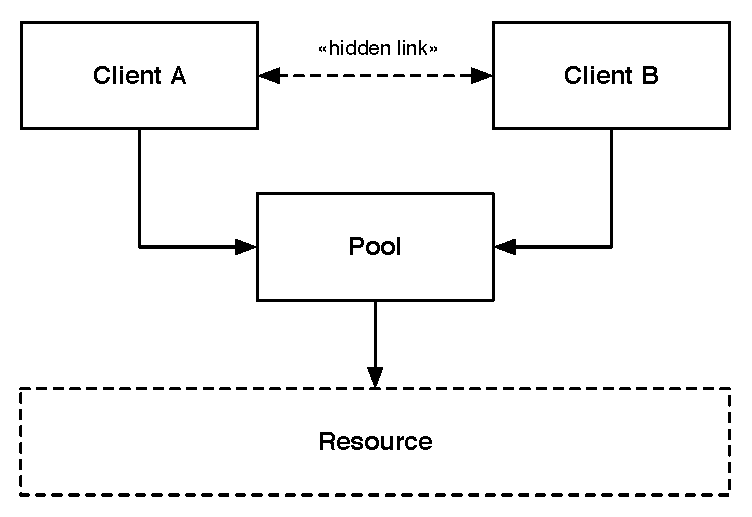
\includegraphics[width=0.5\textwidth]{4-Hauptteil/bulkheads/no-bulkheads.eps}
 \caption{Versteckte Abhängigkeiten durch geteilte Ressourcen.}
 \label{fig:no-bulkheads}
\end{figure}

Die Abbildung zeigt die versteckte Abhängigkeit zwischen den zwei Komponenten, die auf einen gemeinsamen Connection Pool zugreifen \cite[S.~95]{nygard_release_2007}.\\
Angenommen der Client~A hat einen Fehler in der Programmierung und gibt die reservierten Ressourcen, also die Connections nicht wieder frei. Durch den gemeinsam genutzen Connection Pool entwickelt sich der Fehler in der Komponente~A zu einem kaskadierenden Fehler und beeinflusst nun auch Komponente~B \cite[S.~95]{nygard_release_2007} \cite[S.~214]{newman_building_2015}. Der Connection Pool kann der Komponente~B keine freie Connection zuweisen.\\
Ein ähnliches Problem kann entstehen, wenn die Nutzung von Connections in verschiedenen Komponenten unterschiedlich lange dauert. Angenommen Client~A führt ausschließlich schreibende Operationen auf der Connection aus. Client~B hingegen führt ausschließlich lesende Operationen aus. Ferner wird angenommen, dass die schreibenden Operationen schneller ablaufen, als die lesenden Operationen. Dies kann dazu führen, dass Client~B, die schnellere Komponente, von Client~A ausgebremst wird.\\
Gemeinsam benutzte Connection Pools können somit ansonsten isolierte Komponenten beeinflussen und kaskadierende Fehler begünstigen. Es kann also trotz höherer Ressourcenanforderungen Sinn machen, separate Connections Pools für jede Komponente zu nutzen \cite[S.~214]{newman_building_2015}.\\

In jedem dieser Fälle wird deutlich, dass man sich Gedanken über versteckte Abhängigkeiten machen sollte. Das Bulkheads Pattern hilft dabei eine reaktive Anwendung \textit{resilient} zu entwerfen. Jedoch muss das Pattern mit Bedacht angewandt werden. Die Limitierung von Ressourcen, wie etwa die feste Zuweisung von Prozessorkernen kann zu Performanceeinbußen führen. Die Isolation von Komponenten durch separate Connection Pools kann zur überhöhten Ressourcenanforderungen führen. Die Ebene auf der man das Bulkheads Pattern anwendet spielt somit eine Rolle. Zudem ist auch der fachliche Blickwinkel von Bedeutung. Gibt es eine offensichtliche Möglichkeit eines kaskadierenden Fehlers, der das System komplett ausfallen lässt, sollte auf jeden Fall das Bulkheads Pattern in Betracht gezogen werden.

\pagebreak

\subsection{Idempotent Receiver Pattern}\label{subsec:idempotent-receiver-pattern}
Verteilte Anwendungen lassen ihre Komponenten über das Netzwerk miteinander kommunizieren. Eine reaktive Anwendung muss bedingt durch \textit{elasticity} und \textit{resilience} verteilt sein.\\
Bei der Kommunikation über das Netzwerk muss jederzeit mit Ausfällen oder mit verloren gegangenen Nachrichten gerechnet werden. Wie bereits erwähnt, sind Waldo et al. zu dem Schluss gekommen, dass vor allem unvorhersehbare Latenz und teilweiser Ausfall der Kommunikation unvermeidbar sind \cite{waldo_note_1994}. Folglich ist eine garantierte Zustellung einer Nachricht nicht ohne weiteres möglich. Nun stellt sich zudem die Frage was bedeutet \enquote{garantierte Zustellung}?\\
Bedeutet dies, dass die Nachricht\ldots

\begin{enumerate}
\item \ldots in der Message Queue der anderen Komponente angekommen ist,
\item aus der Message Queue entnommen wurde oder
\item erfolgreich verarbeitet wurde \cite{akka_message_2016}?
\end{enumerate}

In jedem Fall muss der Empfänger dem Sender die erfolgreiche Verarbeitung oder den Empfang quittieren. Erst mit der Bestätigungsnachricht kann von einer erfolgreichen Zustellung die Rede sein. Jedoch kann auch die Bestätigungsnachricht auf dem Weg zum Sender verloren gehen (Abb. \ref{fig:failed-ack}) \cite[S.~528]{hohpe_enterprise_2004}.

\begin{figure}[H]
 \centering
 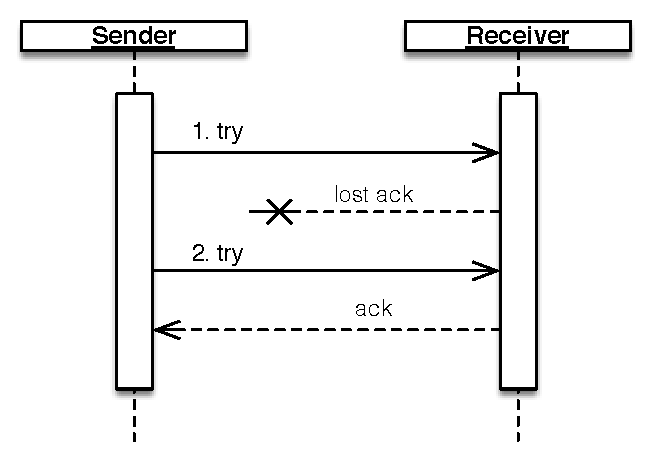
\includegraphics[width=0.54\textwidth]{4-Hauptteil/idempotent-receiver/sequence-failed-ack.eps}
 \caption{Zeitlicher Ablauf einer Kommunikation mit Retry \cite[S.~528]{hohpe_enterprise_2004}.}
 \label{fig:failed-ack}
\end{figure}

Ein beliebtes Mittel, um eine Zustellung zu garantieren, sind Retries im Falle eines Timeouts. Kommt es zu einem Timeout kann der Sender jedoch nicht feststellen, weshalb die Bestätigung nicht eingetroffen ist \cite[S.~382]{vernon_reactive_2016} \cite[S.~528]{hohpe_enterprise_2004}.\\
Die Abbildung \ref{fig:failed-ack} zeigt einen Ablauf in dem die Bestätigungsnachricht beispielsweise durch einen kurzzeitigen Ausfall des Netzwerk verloren ging. Die Zustellung und die Verarbeitung waren erfolgreich, jedoch konnte der Sender nicht informiert werden. Folglich bleibt dem Sender nichts anderes übrig, als die Nachricht erneut zu schicken. Der Empfänger erhält nun zum zweiten Mal die ursprüngliche Nachricht. Angenommen bei der Nachricht handelt es sich um eine Bestellung in einem Onlineshop. Erhält der Empfänger die Nachricht mehrmals, kann dies zu mehrfachen und ungewollten Bestellungen führen.\\
Das Idempotent Receiver Pattern beschreibt die Fähigkeit eines Empfängers mit mehrfach empfangenen und identischen Nachrichten umzugehen. Hohpe und Woolf erklären das Messaging Pattern in ihrem Buch \enquote{Enterprise Integration Patterns} deshalb wie folgt:

\begin{quotation}
Design a receiver to be an Idempotent Receiver, one that can safely receive the same message multiple times \cite[S.~529]{hohpe_enterprise_2004}.
\end{quotation}

Das heißt der Empfänger muss mit Duplikaten einer Nachricht dementsprechend umgehen können, sodass kein fehlerhafter Zustand entsteht.\\
Der mathematische Begriff Idempotenz bedeutet, dass bei der Verknüpfung einer Funktion \textit{f} mit sich selbst folgendes zutrifft \cite[S.~529]{hohpe_enterprise_2004}:
\[f(x) = f(f(x))\]

Analog bedeutet diese Eigenschaft in der Informatik, dass eine Funktion respektive eine Nachricht mehrfach hintereinander ausgeführt werden kann und immer das gleiche Ergebnis liefert.\\

\pagebreak

Die Idempotenz kann im Hinblick auf Nachrichten wie folgt umgesetzt werden \cite[S.~383]{vernon_reactive_2016} \cite[S.~529]{hohpe_enterprise_2004}:

\begin{enumerate}
\item Duplikate werden durch bestimmte Eigenschaften einer Nachricht erkannt und herausgefiltert.
\item Die Zustandsänderung in Folge einer spezifischen Nachricht hat immer die selbe Auswirkung und ist somit \enquote{harmlos} bei mehrfacher Ausführung.
\end{enumerate}

Duplikate einer Nachricht erkennt man am einfachsten durch einen Unique Identifier, also ein eindeutiges Metaattribut --- unabhängig von den eigentlichen Daten. Der Empfänger muss somit eine Liste aller bereits empfangenen bzw. verarbeiteten Nachrichten und deren Unique Identifiers vorhalten. Anhand dieser Liste kann der Empfänger abgleichen, ob eine Nachricht bereits verarbeitet wurde. Hohpe und Woolf schlagen vor, die Liste auf eine gewisse Anzahl von Identifiers zu begrenzen. Als Beispiel erwähnen sie TCP/IP, bei dem es aufgrund von Routing zu Duplikaten von Paketen kommen kann. Bei TCP/IP verständigen sich Sender und Empfänger auf eine maximale Länge dieser Liste \cite[S.~530]{hohpe_enterprise_2004}. Vernon hingegen empfiehlt eine maximale Verweildauer von Einträgen in der Liste zu definieren \cite[S.~383]{vernon_reactive_2016}. Bei Lastspitzen kann es nicht dazu kommen, dass Nachrichten vorzeitig aus der Liste entfernt werden, falls beim Entwurf nicht mit dieser Anzahl von Nachrichten gerechnet wurde.\\

Die zweite Möglichkeit mit Duplikaten umzugehen, ist die Zustandsänderung so zu gestalten, dass es semantisch gesehen keinen Unterschied macht, ob eine Nachricht mehrfach verarbeitet wird \cite[S.~530]{hohpe_enterprise_2004}. Da die Anforderung der garantierten Zustellung einer fachlichen Anforderung zugrunde liegt, ist diese Herangehensweise durchaus sinnvoll. Dadurch ist die Idempotenz nicht an die Nachricht oder an das Messaging System gekoppelt, sondern an die Business Logik. Muss beispielsweise zugesichert werden, dass eine Bestellung maximal einmal ausgeführt wird, sollte jede Bestellung eindeutig durch eine Bestellnummer gekennzeichnet werden. Außerdem sind idempotente Datenstrukturen, wie etwa \textit{Map} in diesem Kontext von Vorteil \cite[S.~386]{vernon_reactive_2016}. Manche Datenbank, wie zum Beispiel PostgreSQL, bieten die Möglichkeit anhand einer Bedingung ein \textit{UPDATE} Statement anstatt eines \textit{INSERT} Statements durchzuführen, um Konflikte durch mehrfache Ausführung zu umgehen. Dies wird meist als \textit{UPSERT} bezeichnet\footnote{https://wiki.postgresql.org/wiki/UPSERT}.\\

Komponenten bei denen eine garantierte Zustellung und somit eine Bestätigungsnachricht erforderlich ist, sollten als Idempotent Receiver implementiert werden. Dieses Vorgehen wird sowohl von Akka als auch Vert.x empfohlen. Durch das Pattern ist es möglich, die einfache Fehlerbehandlung durch Retries umzusetzen ohne dabei einen fehlerhaften Zustand zu erzeugen. Wichtig ist auch, dass sich die Idempotenz auf den Zustand der Business Logik bezieht --- es spricht beispielsweise nichts dagegen mehrfache Anfragen zu protokollieren \cite[S.~216]{newman_building_2015}.

\pagebreak

\subsection{Saga Pattern}\label{subsec:saga-pattern}
Durch das Simple Component Pattern und durch die Isolation der Komponenten sind die Daten eines reaktiven Systems verteilt. Im Vergleich zu einer traditionellen Anwendung mit lediglich einer Datenbank ist es aufwendig und kompliziert eine Transaktion mit mehreren verteilten Komponenten durchzuführen.\\
Bestimmte Anwendungsfälle fordern Konsistenz über mehrere verteile Komponenten hinweg. Solche Anwendungsfälle beschreiben meist mehrere Aktionen von denen entweder alle oder im Fehlerfall keine eine Auswirkung haben sollte. Für gewöhnlich greift man in diesen Fällen zu Shared Locks und Protokollen wie Two-Phase Commit --- oder allgemein zu verteilten Transaktionen \cite{mccaffrey_goto_2015}. Jedoch sind verteilte Transaktionen Ressourcen intensiv und kompliziert zu implementieren. Die involvierten Komponenten einer verteilten Transaktion sind nicht mehr lose gekoppelt und teilweise voneinander abhängig.\\
Das Saga Pattern erfüllt die Anforderung der Konsistenz ohne komplizierte und verteilte Transaktionen. Der Begriff \enquote{Saga} wurde durch Garcia-Molina und Salem in deren Artikel \enquote{SAGAS} geprägt \cite{garcia-molina_sagas_1987}. In dem Artikel wird beschrieben, wie langlebige Transaktionen in mehrere fachliche Teiltransaktionen aufgeteilt werden können. Das ist erstrebenswert, da langlebige Transaktionen ebenso lange Ressourcen durch Locks blockieren. Durch die Verwendung von Transaktionen wird Atomicity und Consistency sichergestellt. Jedoch werden nebenläufige Transaktionen, welche auf die selben Daten zugreifen, durch Wartezeiten oder gar Deadlocks negativ beeinflusst. Bei langlebigen und großen Transaktionen trifft dies umso mehr zu, denn diese binden meist viele Ressourcen an sich \cite[S.~307]{kuhn_reactive_2015}.\\
Teilt man eine große Transaktion in mehrere fachliche Teiltransaktionen auf verliert man die Eigenschaften Atomicity und Consistency. Denn nach jeder abgeschlossenen Teiltransaktion sind deren Änderungen persistent und für andere Teilnehmer sichtbar und somit nicht mehr atomar. Bricht eine der Teiltransaktionen aufgrund eines Fehlers ab, werden die bereits beendeten Teiltransaktionen nicht durch den Rollback zurückgenommen. Dies kann zu einem inkonsistenen Zustand \mbox{führen}.

\pagebreak

Garcia-Molina und Salem argumentieren, dass für bestimmte Anwendungsfälle lediglich die Consistency gewahrt werden muss und die Atomicity vernachlässigt werden kann \cite[S.~250]{garcia-molina_sagas_1987}. Um zu einem Konsens zu gelangen müssen entweder alle oder keine der Teiltransaktionen eine Auswirkung haben \cite[S.~250]{garcia-molina_sagas_1987}. Deshalb definiert eine Saga nicht nur eine Abfolge von Teiltransaktionen \textit{T} sondern auch eine Abfolge von zugehörigen Ausgleichstransaktionen \textit{C}. Die Ausgleichstransaktion \textit{C\textsubscript{n}} macht die fachlichen Auswirkungen der Teiltransaktion \textit{T\textsubscript{n}} rückgängig. Ist eine Teiltransaktion fehlerhaft, werden von allen bis dahin ausgeführten Teiltransaktionen deren Ausgleichstransaktionen ausgeführt. Somit wird trotz Fehlerfall und der Ausführungen einzelner Transaktionen die Consistency gewahrt.\\
Angenommen in einer Abfolge von vier Teiltransaktionen schlägt die Teiltransaktion \textit{T\textsubscript{3}} fehl. Der Ablauf der Ausführung sähe dann folgendermaßen aus:

\begin{quotation}
\textit{T\textsubscript{1}} $\rightarrow$ \textit{T\textsubscript{2}} $\rightarrow$ \textit{T\textsubscript{3}}\,\textdagger\,$\rightarrow$ \textit{C\textsubscript{3}} $\rightarrow$ \textit{C\textsubscript{2}} $\rightarrow$ \textit{C\textsubscript{1}}
\end{quotation}

Um einen konsistenen Zustand zu hinterlassen, werden die Ausgleichstransaktionen \textit{C\textsubscript{3}}--\textit{C\textsubscript{1}} in umgekehrter Reihenfolge zu deren Teiltransaktionen ausgeführt. Die Zustandsänderungen von \textit{T\textsubscript{1}}--\textit{T\textsubscript{3}} werden sematisch zurückgenommen. Da die Teiltransaktion \textit{T\textsubscript{4}} nicht ausgeführt wurde, wird auch deren Ausgleichstransaktion \textit{C\textsubscript{4}} nicht ausgeführt.\\

Das Prinzip einer Saga lässt sich sehr gut auf ein reaktives System und die Kommunikation zwischen mehreren Komponenten übertragen. Nicht selten kommt es vor, dass eine Anfrage mehrere Zustandsänderungen --- also Teiltransaktionen --- in verschiedenen Komponenten bewirkt. Kuhn beschreibt deshalb eine Saga im Bezug auf reaktive Systeme mit folgenden zwei Sätzen:

\begin{quotation}
Divide long-lived distributed transactions into quick local ones with compensating actions for recovery. [Therefore] create an ephemeral component to manage the execution of a sequence of actions distributed across multiple components \cite[S.~307]{kuhn_reactive_2015}.
\end{quotation}

In einem reaktiven System wird eine Saga somit von einer Anfrage ausgelöst. Diese Anfrage zieht mehrere Unter- bzw.Teilanfragen anstelle von Teiltransaktionen nach sich. Zu jeder Teilanfrage wird eine Ausgleichsanfrage definiert \cite{mccaffrey_goto_2015}.\\
Folgendes Sequenzdiagramm zeigt einen möglichen Ablauf einer Saga in einem verteilten System mit mehreren unabhängigen Komponenten. Das Beispiel zeigt einen Onlineshop bei dem aufgrund einer Bestellung drei weitere Komponenten angefragt werden. Der Kunde bestätigt seinen Einkauf und schickt die Bestellung ab. Die Ordering Komponente informiert drei weitere Komponenten --- wovon jedoch eine die Teilanfrage nicht bearbeiten kann. Nun werden die Ausgleichanfragen der Saga ausgeführt.

\begin{figure}[H]
 \centering
 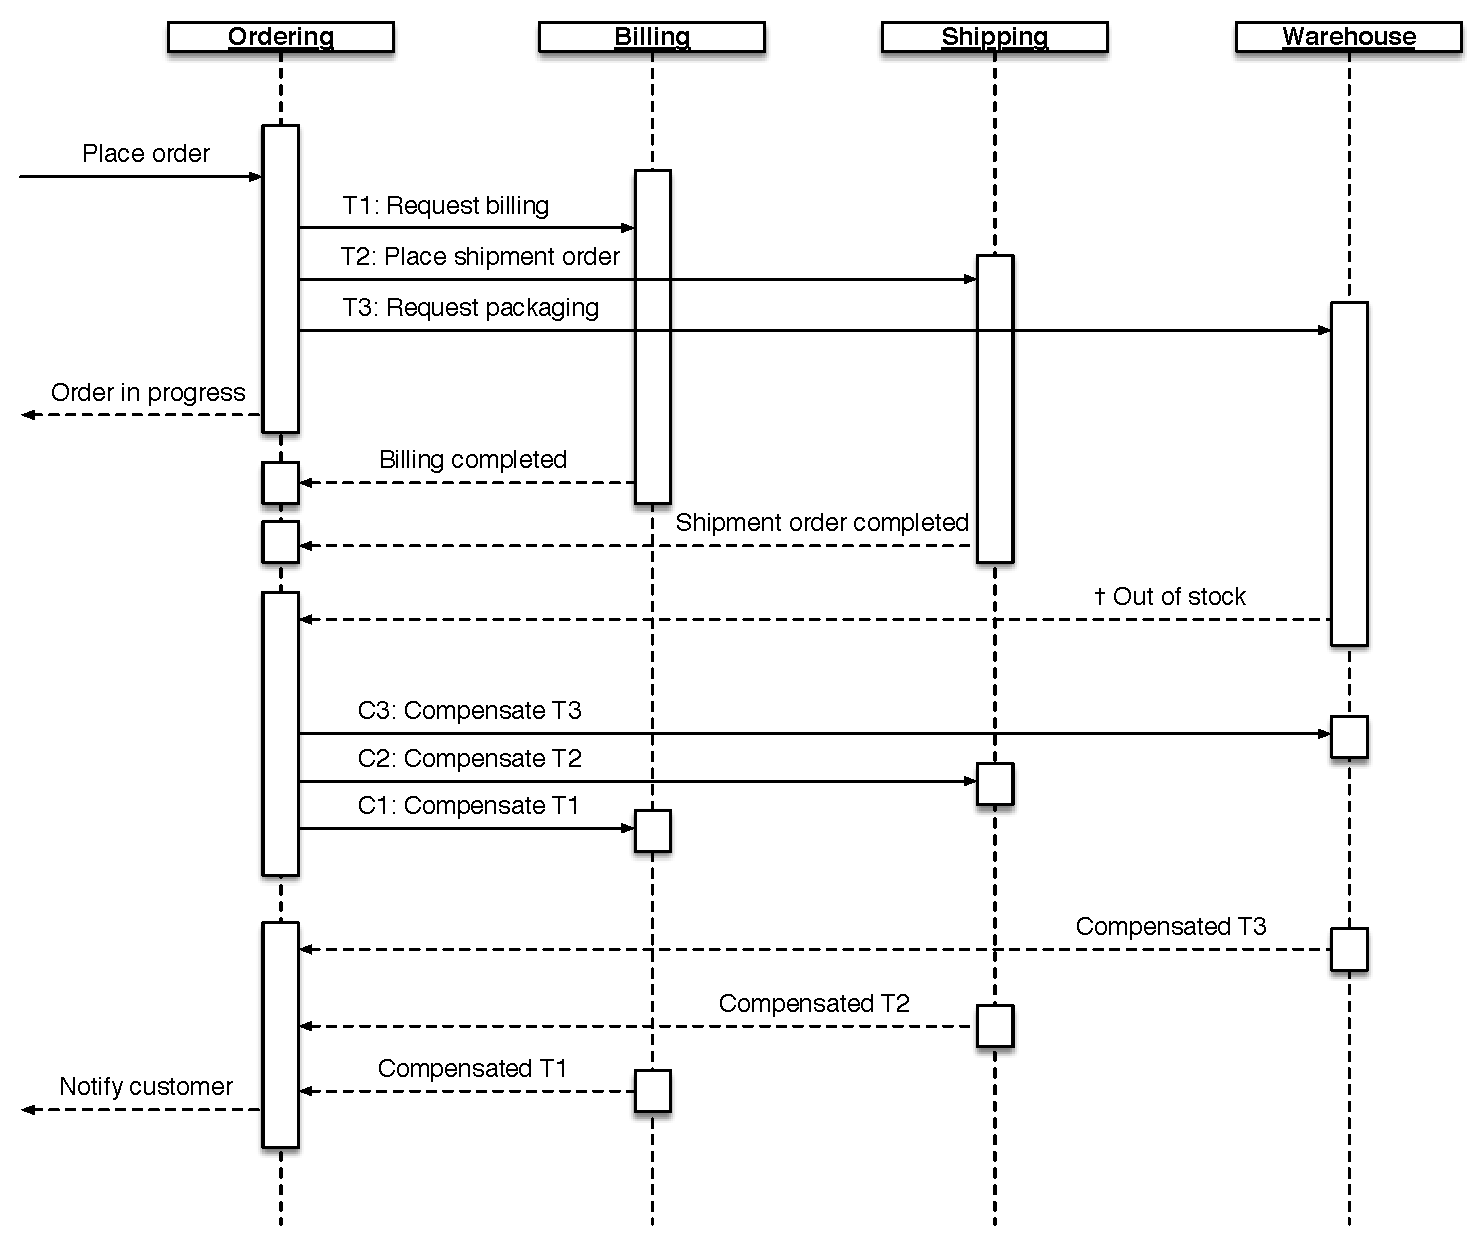
\includegraphics[width=1\textwidth]{4-Hauptteil/saga/onlineshop-saga.eps}
 \caption{Zeitlicher Ablauf einer Saga mit einer fehlerhaften Unteranfrage.}
 \label{fig:sequence-saga}
\end{figure}

\pagebreak

Die Komponente, die die Saga initiert und koordiniert wird Saga Execution Coordinator genannt. Es empfiehlt sich die Koordination in eine eigene kleine Komponente auszulagern. Die einzelnen Schritte einer Saga müssen protokolliert und persistiert werden. Dies ist nötigt, da der Saga Execution Coordinator selbst ausfallen kann. In dem sogenannten Saga Log werden Beginn und Ende der Teilanfragen sowie Beginn und Ende der Saga protokolliert. Auch die im Fehlerfall ausgeführten Ausgleichsanfragen werden festgehalten. Mit dem Beginn der Saga müssen für den Saga Execution Coordinator alle benötigten Informationen für die Ausführung der Saga zur Verfügung stehen. Anhand des Logs kann der Execution Coordinator, beispielsweise nach einen unvorhergesehenen Neustart, erkennen in welchen Zustand die Saga ist und welche weiteren Maßnahmen ergriffen werden müssen.\\
Um einen garantierten und sicheren Zustand nach einer fehlerhaften Saga zuerhalten, müssen die Ausgleichsanfragen bzw. deren Empfänger das Idempotent Receiver Pattern (\ref{subsec:idempotent-receiver-pattern}) implementieren \cite{mccaffrey_goto_2015}. Zudem empfiehlt es sich die Teilanfragen ebenfalls idempotent umzusetzen. Sind alle Anfragen idempotent kann eine Saga oder die fehlerhaften Teile einer Saga erneut ausgeführt werden bis alle Teilanfragen oder alle nötigen Ausgleichsanfragen erfolgreich beendet wurden.\\

Das Saga Pattern hilft dabei langlebige und verteilte Aktionen in einer reaktiven Anwendung umzusetzen. Es lässt sich sehr gut mit dem Simple Component Pattern und der daraus resultierenden Isolation von Komponenten und deren Daten vereinen. Im Vergleich zu Protokollen mit Two-Phase Commit werden keine Shared Locks benötigt und die \textit{responsiveness} des Systems wird nicht eingeschränkt. Aufgrund der expliziten Definition der ausgleichenden Maßnahmen kann das Saga Pattern als Failure Management Pattern gesehen werden \cite{mccaffrey_goto_2015}. Es eignet sich jedoch nur für Anwendungsfälle deren Business Logik keine atomare und isolierte Aktion vorschreibt. Trotz der Einschränkung können viele reale Anwendungsfälle mit dem Saga Pattern effizient umgesetzt werden.
